\documentclass[tikz,border=8pt]{standalone}
\usepackage[T1]{fontenc}
\usepackage{lmodern}
\usepackage{amsmath,amssymb}
\pdfinfoomitdate=1
\pdfsuppressptexinfo=-1
\pdftrailerid{}
\usepackage{hyperref}
\usetikzlibrary{arrows.meta,calc}

\definecolor{ink}{HTML}{203044}
\definecolor{blue}{HTML}{2E627D}
\definecolor{green}{HTML}{346C59}
\definecolor{purple}{HTML}{62517C}
\definecolor{muted}{HTML}{5E6874}
\hypersetup{colorlinks=true,urlcolor=blue,
  pdftitle={I3322: paper-to-Lean proof map},
  pdfauthor={},pdfcreator={},pdfproducer={},pdfsubject={},pdfkeywords={}}
\newcommand{\module}[1]{{\color{muted}\fontsize{9.4}{12}\selectfont\texttt{#1}}}
\newcommand{\decl}[1]{{\fontsize{8.6}{11}\selectfont\texttt{#1}}}
\newcommand{\betapv}{\beta_{\mathrm{PV}}}
\tikzset{
  every picture/.style={font=\fontsize{10.5}{13}\selectfont,text=ink,
    >=Latex,line cap=round,line join=round},
  box/.style={draw=blue,line width=.7pt,fill=blue!4,rounded corners=2pt,
    align=center,text width=6.7cm,inner xsep=6pt,inner ysep=6pt,
    minimum height=1.6cm},
  result/.style={box,draw=purple,fill=purple!6,line width=1pt},
  strict/.style={box,draw=green,fill=green!5},
  repeat/.style={box,fill=white},
  dependency/.style={draw=ink!75,line width=.7pt,
    -{Latex[length=2.1mm,width=1.5mm]},rounded corners=3pt},
  bus/.style={draw=ink!75,line width=.7pt,rounded corners=3pt},
  note/.style={align=left,text=muted,font=\fontsize{9.2}{12}\selectfont}
}

\begin{document}
\pagecolor{white}
\hyphenpenalty=10000
\exhyphenpenalty=10000
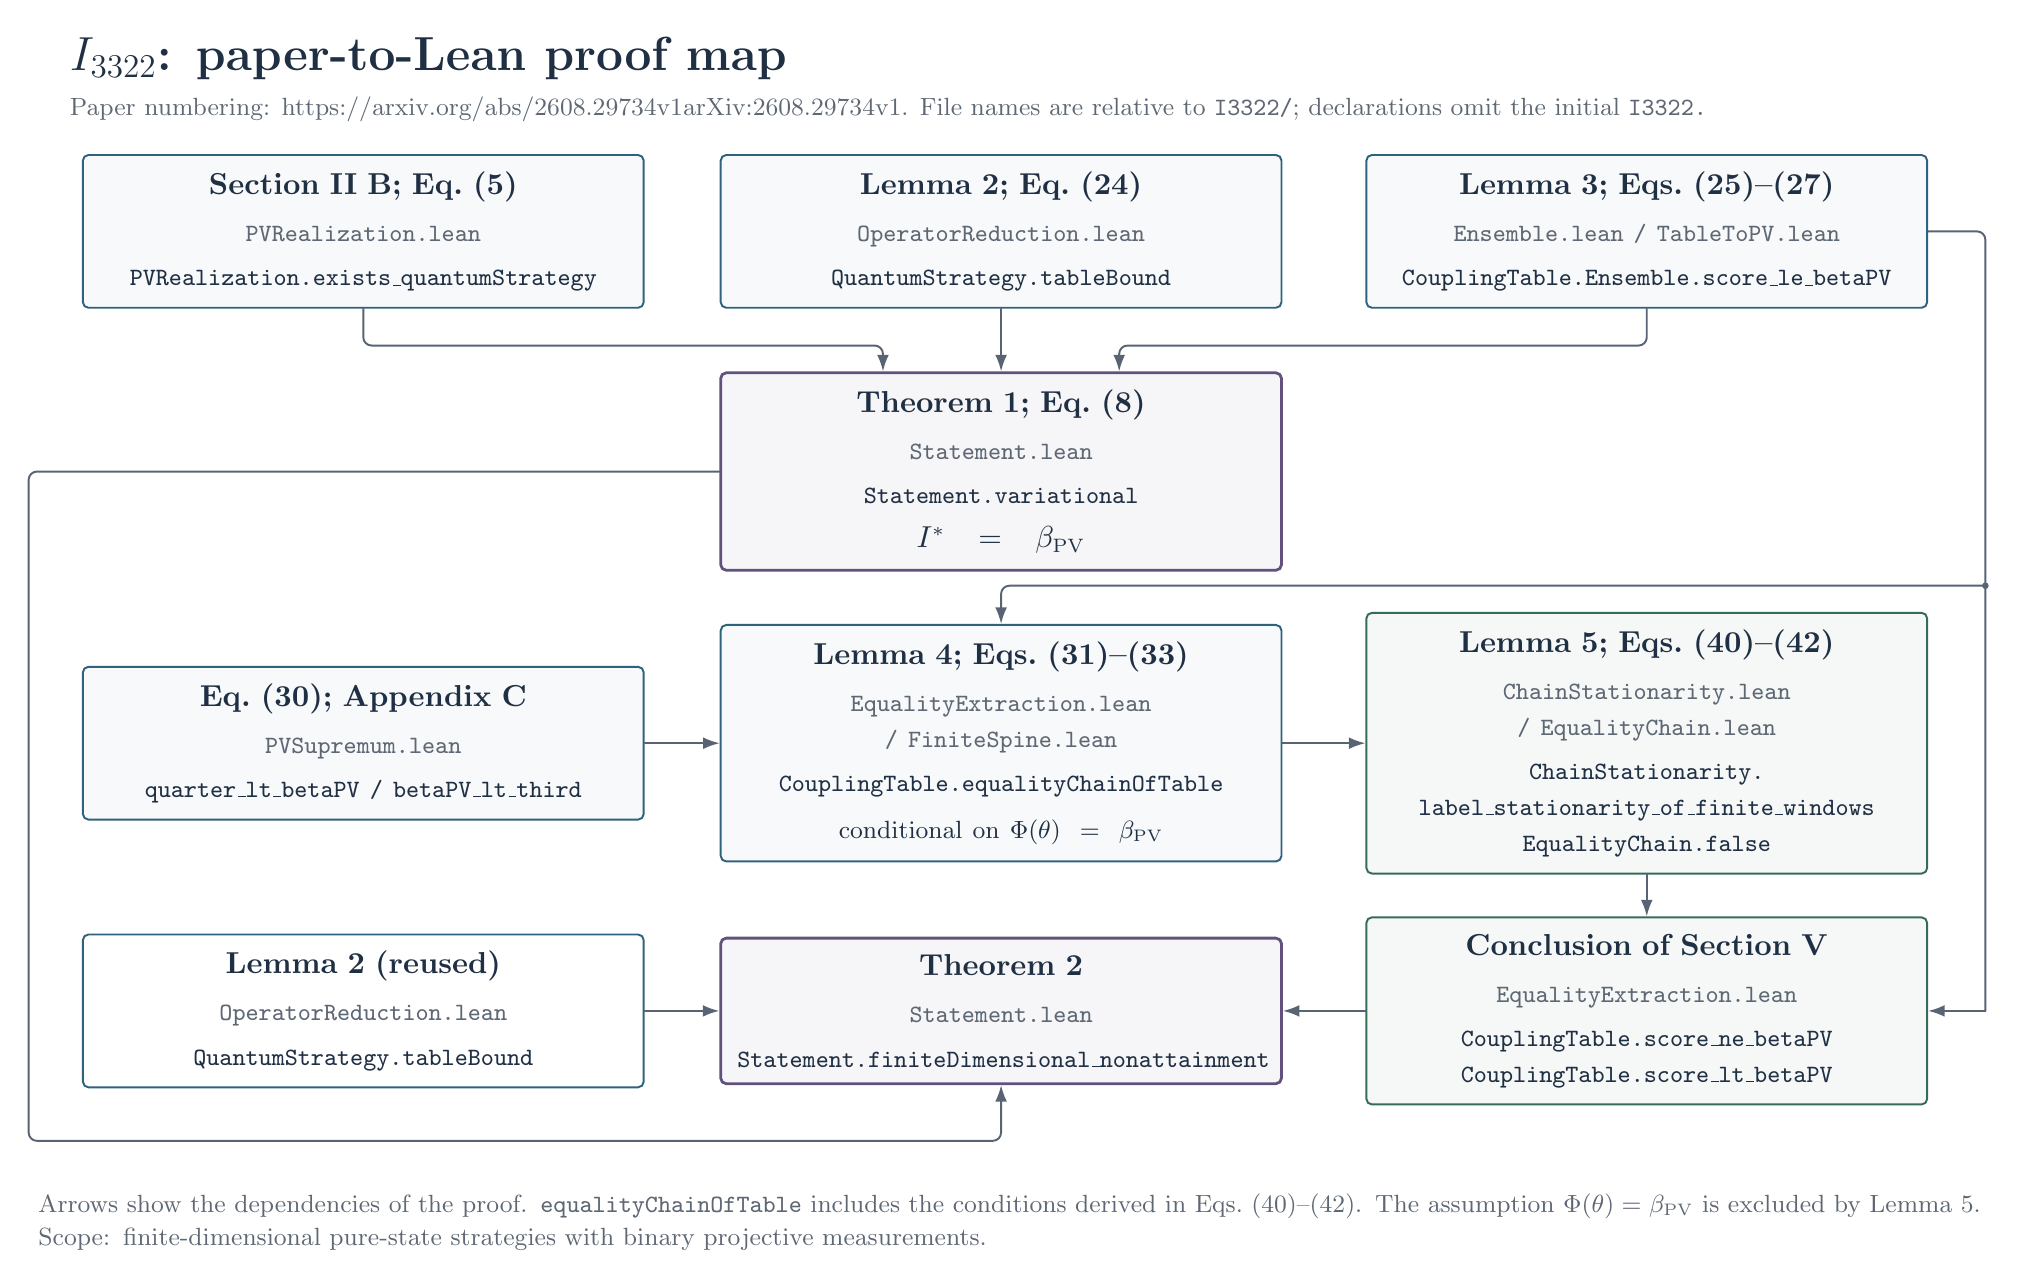
\begin{tikzpicture}[x=1cm,y=1cm]
  \node[anchor=west,font=\fontsize{17}{20}\selectfont\bfseries]
    at (-.15,2.20) {$I_{3322}$: paper-to-Lean proof map};
  \node[anchor=west,note] at (-.15,1.55)
    {Paper numbering: \href{https://arxiv.org/abs/2608.29734v1}{arXiv:2608.29734v1}.
     File names are relative to \texttt{I3322/}; declarations omit the initial \texttt{I3322.}};

  \node[box] (realization) at (3.7,0)
    {\textbf{Section II B; Eq.\ (5)}\\[4pt]
     \module{PVRealization.lean}\\[3pt]
     \decl{PVRealization.exists\_quantumStrategy}};

  \node[box] (operator) at (11.8,0)
    {\textbf{Lemma 2; Eq.\ (24)}\\[4pt]
     \module{OperatorReduction.lean}\\[3pt]
     \decl{QuantumStrategy.tableBound}};

  \node[box] (table) at (20.0,0)
    {\textbf{Lemma 3; Eqs.\ (25)--(27)}\\[4pt]
     \module{Ensemble.lean / TableToPV.lean}\\[3pt]
     \decl{CouplingTable.Ensemble.score\_le\_betaPV}};

  \node[result] (identity) at (11.8,-3.05)
    {\textbf{Theorem 1; Eq.\ (8)}\\[4pt]
     \module{Statement.lean}\\[3pt]
     \decl{Statement.variational}\\[3pt]
     $I^*=\betapv$};

  \draw[dependency] (realization.south) -- (3.7,-1.45)
    -- (10.3,-1.45) -- ([xshift=-1.5cm]identity.north);
  \draw[dependency] (operator.south) -- (identity.north);
  \draw[dependency] (table.south) -- (20.0,-1.45)
    -- (13.3,-1.45) -- ([xshift=1.5cm]identity.north);

  \node[box] (enclosure) at (3.7,-6.50)
    {\textbf{Eq.\ (30); Appendix C}\\[4pt]
     \module{PVSupremum.lean}\\[3pt]
     \decl{quarter\_lt\_betaPV / betaPV\_lt\_third}};

  \node[box] (extraction) at (11.8,-6.50)
    {\textbf{Lemma 4; Eqs.\ (31)--(33)}\\[4pt]
     \module{EqualityExtraction.lean / FiniteSpine.lean}\\[3pt]
     \decl{CouplingTable.equalityChainOfTable}\\[4pt]
     {\fontsize{9.2}{11}\selectfont conditional on $\Phi(\theta)=\betapv$}};

  \node[strict] (contradiction) at (20.0,-6.50)
    {\textbf{Lemma 5; Eqs.\ (40)--(42)}\\[4pt]
     \module{ChainStationarity.lean / EqualityChain.lean}\\[3pt]
     \decl{ChainStationarity.}\\
     \decl{label\_stationarity\_of\_finite\_windows}\\
     \decl{EqualityChain.false}};

  \draw[dependency] (enclosure.east) -- (extraction.west);
  \draw[dependency] (extraction.east) -- (contradiction.west);

  \draw[bus] (table.east) -- (24.3,0) -- (24.3,-9.9);
  \draw[dependency] (24.3,-4.50) -- (11.8,-4.50) -- (extraction.north);
  \fill[ink!75] (24.3,-4.50) circle (1.2pt);

  \node[repeat] (operatorAgain) at (3.7,-9.90)
    {\textbf{Lemma 2 (reused)}\\[4pt]
     \module{OperatorReduction.lean}\\[3pt]
     \decl{QuantumStrategy.tableBound}};

  \node[strict] (strictness) at (20.0,-9.90)
    {\textbf{Conclusion of Section V}\\[4pt]
     \module{EqualityExtraction.lean}\\[3pt]
     \decl{CouplingTable.score\_ne\_betaPV}\\
     \decl{CouplingTable.score\_lt\_betaPV}};

  \node[result] (nonattainment) at (11.8,-9.90)
    {\textbf{Theorem 2}\\[4pt]
     \module{Statement.lean}\\[3pt]
     \decl{Statement.finiteDimensional\_nonattainment}};

  \draw[dependency] (contradiction.south) -- (strictness.north);
  \draw[dependency] (24.3,-9.90) -- (strictness.east);
  \draw[dependency] (strictness.west) -- (nonattainment.east);
  \draw[dependency] (operatorAgain.east) -- (nonattainment.west);
  \draw[dependency] (identity.west) -- (-.55,-3.05)
    -- (-.55,-11.55) -- (11.8,-11.55) -- (nonattainment.south);

  \node[note,anchor=north west,text width=24.7cm] at (-.55,-12.1)
    {Arrows show the dependencies of the proof.
     \texttt{equalityChainOfTable} includes the conditions derived in
     Eqs.\ (40)--(42). The assumption $\Phi(\theta)=\betapv$ is excluded by
     Lemma 5. Scope: finite-dimensional pure-state strategies with binary
     projective measurements.};
\end{tikzpicture}
\end{document}
